\section{Environnement de travail \& solutions retenues}
Je ne suis intervenu que sur des projets qui étaient déjà commencés, et de ce fait il n'y a eu que peu de choix en termes de solutions retenues. Je vais néanmoins détailler ici l'environnement de travail, les différentes solutions techniques qui étaient déjà en place à mon arrivée et avec lesquelles j'ai travaillé pendant 6 mois.

Pour autant, il est intéressant de résumer l'environnement dans lequel j'ai évolué pendant 6 mois, pour chacun des pans très variés sur lesquels je suis intervenu. Les sous-sections seront volontairement brèves ; plus de détails seront disponibles dans les parties~\ref{sec:synthese_ci},~\ref{sec:synthese_java} et~\ref{sec:synthese_audit}.

\subsection{CI}
\subsubsection{GitLab \& GitLab-CI}
L'intégration continue dans les projets d'Alter Frame se fait à l'aide d'un service proposé par la plateforme d'hébergement de projets informatiques GitLab\cite{gitlab}. Le service en question, GitLab-CI\cite{gitlab-ci}, propose de mettre en place de l'intégration continue sur les projets hébergés sur GitLab.

Au moment de mon arrivée chez Alter Frame la partie CI des projets consistait majoritairement en la compilation des projets et une analyse de code à l'aide d'un plugin SonarQube\cite{sonarqube}, mise en place depuis environ 2 ans.

Le principe est que les actions décrites ci-dessus, compilation et analyse de code, sont effectuées à chaque push sur le serveur GitLab. Ce fonctionnement peut ensuite être affiné, pour ne se produire que lorsqu'un tag git est pushé ou sur certaines branches (branche master, tag de release, etc).

Il n'y avait néanmoins pas de composante cybersécurité dans le processus de CI d'Alter Frame et c'est donc ce sur quoi je suis intervenu en priorité. Néanmoins, mon travail ne s'est pas limité à cela et j'ai aussi pu intervenir sur d'autres aspects du CI et améliorer l'existant.

\subsubsection{ZAP : Zed Attack Proxy}
\begin{figure}
	{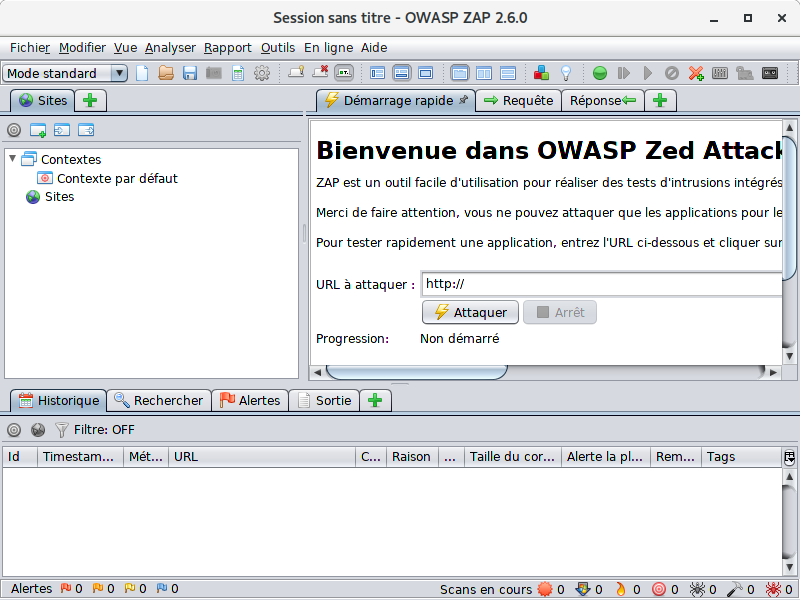
\includegraphics[width=\textwidth]{images/zap_acceuil}}
	\centering
	\caption{Fenêtre de démarrage de ZAP}
	\label{fig:zap_acceuil}
\end{figure}
ZAP\cite{zap} (voir figure~\ref{fig:zap_acceuil}) est un projet open source développé par l'OWASP\cite{owasp}. Il s'agit un proxy qui peut intercepter et analyse le trafic qui traverse la machine hôte. ZAP est un outil de sécurité très intéressant et ce pour un grand nombre de raisons :
\begin{itemize}
	\item activement développé\cite{zap_git} ;
	\item open source et cross-platform ;
	\item OWASP est une référence dans le monde de la sécurité ;
	\item une large communauté, et donc une grande quantité de ressources sur laquelle s'appuyer ;
	\item ZAP est contrôlable en ligne de commande (voir extrait~\ref{lst:zap_options}) et \textit{via} des APIs en plusieurs langages.
\end{itemize}

\begin{minipage}{\linewidth}
	\begin{lstlisting}[caption={Options de ZAP en ligne de commande},label={lst:zap_options},numbers=none]
$ zap.sh -cmd -help
Usage:
    zap.sh [Options]
Core options:
    -version                 Reports the ZAP version
    -cmd                     Run inline (exits when command line options complete)
    -daemon                  Starts ZAP in daemon mode, ie without a UI
    -config <kvpair>         Overrides the specified key=value pair in the configuration file
    -configfile <path>       Overrides the key=value pairs with those in the specified properties file
    -dir <dir>               Uses the specified directory instead of the default one
    -installdir <dir>        Overrides the code that detects where ZAP has been installed with the specified directory
    -h                       Shows all of the command line options available, including those added by add-ons
    -help                    The same as -h
    -newsession <path>       Creates a new session at the given location
    -session <path>          Opens the given session after starting ZAP
    -host <host>             Overrides the host used for proxying specified in the configuration file
    -port <port>             Overrides the port used for proxying specified in the configuration file
    -lowmem                  Use the database instead of memory as much as possible - this is still experimental
    -experimentaldb          Use the experimental generic database code, which is not surprisingly also still experimental
    -nostdout                Disables the default logging through standard output
Add-on options:
    -script <script>         Run the specified script from commandline or load in GUI
    -addoninstall <addon>    Install the specified add-on from the ZAP Marketplace
    -addoninstallall         Install all available add-ons from the ZAP Marketplace
    -addonuninstall <addon>  Uninstall the specified add-on
    -addonupdate             Update all changed add-ons from the ZAP Marketplace
    -addonlist               List all of the installed add-ons
    -quickurl [target url]: The URL to attack, eg http://www.example.com
    -quickout [output filename]: The file to write the XML results to
    -quickprogress: Display progress bars while scanning
    -last_scan_report <path> Generate the 'Last Scan Report' into the specified path
\end{lstlisting}
\end{minipage}

Je n'avais, avant mon stage, que brièvement eu l'occasion d'utiliser ZAP, au-travers du sous-projet de tests d'intrusion avec M. Pachy. Pouvoir m'entraîner plus longuement avec représentait donc à la fois un intérêt personnel, car cela me permettait d'en apprendre plus sur les vulnérabilités web les plus répandues, et professionnel car c'est un outil dont l'usage pourrait être pertinent pour mes futurs emplois.

ZAP est le seul outil sur lequel il y a vraiment eu un choix à faire car les tests de sécurité n'étaient pas encore implémentés à mon arrivée. Le principal concurrent de ZAP est Burp Suite\cite{burp}, une solution non-libre mais qui dispose d'une version gratuite.

Les arguments qui ont fait pencher la balance en la faveur de ZAP sont :
\begin{itemize}
	\item le fait que l'OWASP est une référence dans le monde de la sécurité ;
	\item le développement ouvert qui est une assurance de qualité dans le monde de la sécurité (possibilité de relever les failles/oublis/erreurs dans le code) ;
	\item le fait que moi comme mon tuteur ayons déjà eu une expérience avec ZAP et pas avec Burp.
\end{itemize}

\subsubsection{Docker}
Docker\cite{docker} est une technologie de virtualisation basée sur des conteneurs, qui vient se place en opposition aux hyperviseurs et machines virtuelles\footnote{Ou VMs pour Virtual Machines}. En plus d'une charte graphique à base de faune marine des plus plaisantes\footnote{\url{https://www.docker.com/sites/default/files/group_5622_0.png}}, la technologie Docker présente plusieurs fonctionnalités qui la rendent intéressante dans le monde de l'industrie informatique :
\begin{itemize}
	\item un conteneur est plus léger qu'une VM ;
	\item un conteneur s'exécute de la même façon sur n'importe quelle machine où Docker est installé ;
	\item un conteneur peut embarquer toute la configuration nécessaire au bon fonctionnement de l'application, et c'est là le point le plus important. L'étape de configuration de l'environnement n'a à être effectuée qu'une seule fois, à la création de l'image\footnote{On ne parle de conteneur qu'une fois l'image en cours d'exécution, cf. différence entre processus et programme}. De plus le système de Docker Store\cite{docker_store}, proche de celui d'un gestionnaire de paquets, permet au client d'avoir facilement la dernière version possible d'un logiciel, encore une fois en s'abstrayant des changements de configuration qui vont avec la mise-à-jour.
\end{itemize}

On assiste donc à une généralisation de l'utilisation de Docker depuis sa première version en 2013, avec de nombreux cas d'utilisation\cite{docker_use_cases}, mais aussi à une multiplication des outils en lien avec la technologie Docker comme des outils de gestion de groupes de containers\cite{kubernetes}\cite{swarm}.

GitLab-CI est étroitement lié à Docker : lors d'un push, un container est lancé dans lequel tout le processus de CI est exécuté, en isolation. De ce fait, il n'y avait pas de choix à faire quant à la technologie de virtualisation. Le comportement du processus peut être configuré au-travers d'un script en YAML, il est par exemple possible de sélectionner l'image Docker servant d'environnement d'exécution.

\subsubsection{YAML}
YAML Ain't Markup Language\cite{yaml}, de son nom complet, est un \og standard de sérialisation de données \fg. L'objectif de ce langage est de permettre de représenter des donnes à la fois clairement et simplement, principalement en les formatant comme des listes ou des maps.

La syntaxe de YAML est donc sans surprise concise et facile de prise en main\cite{yaml_refcard} ; qui plus est le code YAML est assez proche de l'anglais pour être compréhensible même par quelqu'un qui n'y est pas familier.

Dans le cas qui nous occupe, YAML est le langage permettant de contrôler le processus de CI proposé par GitLab-CI grâce à un script nommé \verb|.gitlab-ci.yml| placé à la racine du projet (l'extrait~\ref{lst:yaml_ci} est un exemple écourté de script YAML sur lequel j'ai travaillé).

\begin{minipage}{\linewidth}
	\begin{lstlisting}[caption={Script de contrôle de processus de CI en YAML},label={lst:yaml_ci}]
variables:
    MYSQL_DATABASE: database_name

services:
    - mysql:latest
    - redis:latest

deploy:
    stage: build
    image: aleonardi/symfony-mysqlclient
    stage: build
    script:
        - bash .gitlab-ci.sh
        - chmod a+x vendor/bin/phpunit
        - php vendor/bin/phpunit --colors

zap-docker:
    stage: test
    image: owasp/zap2docker-weekly:latest
    script:
        - python zap-baseline.py -t http://rick.alter-frame.fr/ -c zap.conf
    artifacts:
        - ./zap-report
    only:
        - master
        - tags
    \end{lstlisting}
\end{minipage}

\subsection{Développement Java}
Il y a moins à dire sur le développement Java car il s'agit d'un pan de travail très proche de ce que j'ai déjà rencontré par le passé, que ce soit dans des cours ou dans mon précédent stage. Chez Alter Frame, j'ai développé en Java 7 couplé à Swing pour la GUI, le tout dans un environnement Windows en utilisant les classiques Maven et git.

Encore une fois, le projet ne m'ayant pas attendu pour en premier lieu, il n'y avait pas de grande marge de manoeuvre quand à quelles technologies utiliser. L'environnement Windows est indépendant de Java à proprement parler, mais dû à l'utilisation de VBScript pour créer et modifier des classeurs Microsoft Excel.

L'incompatibilité entre le projet et Java 8 reste, elle, un mystère\footnote{\url{https://i.pinimg.com/564x/66/ba/a0/66baa08b16a192d752959fa4c29bc96a.jpg}}.
%\footnote{\url{https://xkcd.com/722/}}.

\subsection{Audit technique}
\subsubsection{ZAP : Zed Attack Proxy}
J'ai à nouveau eu l'occasion d'utiliser ZAP pendant le déroulement de l'audit. Cette fois-ci il ne s'agissait pas d'en automatiser l'usage et donc de le contrôler au-travers d'une API, mais bien d'un cas d'usage plus classique où j'ai configuré ZAP comme proxy Internet, et observé le trafic lors de l'utilisation de l'application auditée grâce à son interface graphique.

Néanmoins, les avantages de ZAP qui ont fait que mon tuteur et moi l'avons retenu pour l'intégration continue s'appliquent toujours ici (excepté pour le contrôle par API/ligne de commande) et le raison du choix de ZAP est donc la même.

\subsubsection{SonarQube}
SonarQube est un outil d'analyse de code bien connu. Bien que sa vocation première soit d'améliorer la qualité et la maintenabilité du code analysé, Sonar incorpore aussi des règles de sécurité dans ses patrons de détection. C'est dans cette optique que je l'ai utilisé (la figure~\ref{fig:sonar_sec} liste une partie des vulnérabilités que sait détecter Sonar).

\begin{figure}{l}
	\makebox[\textwidth][c]{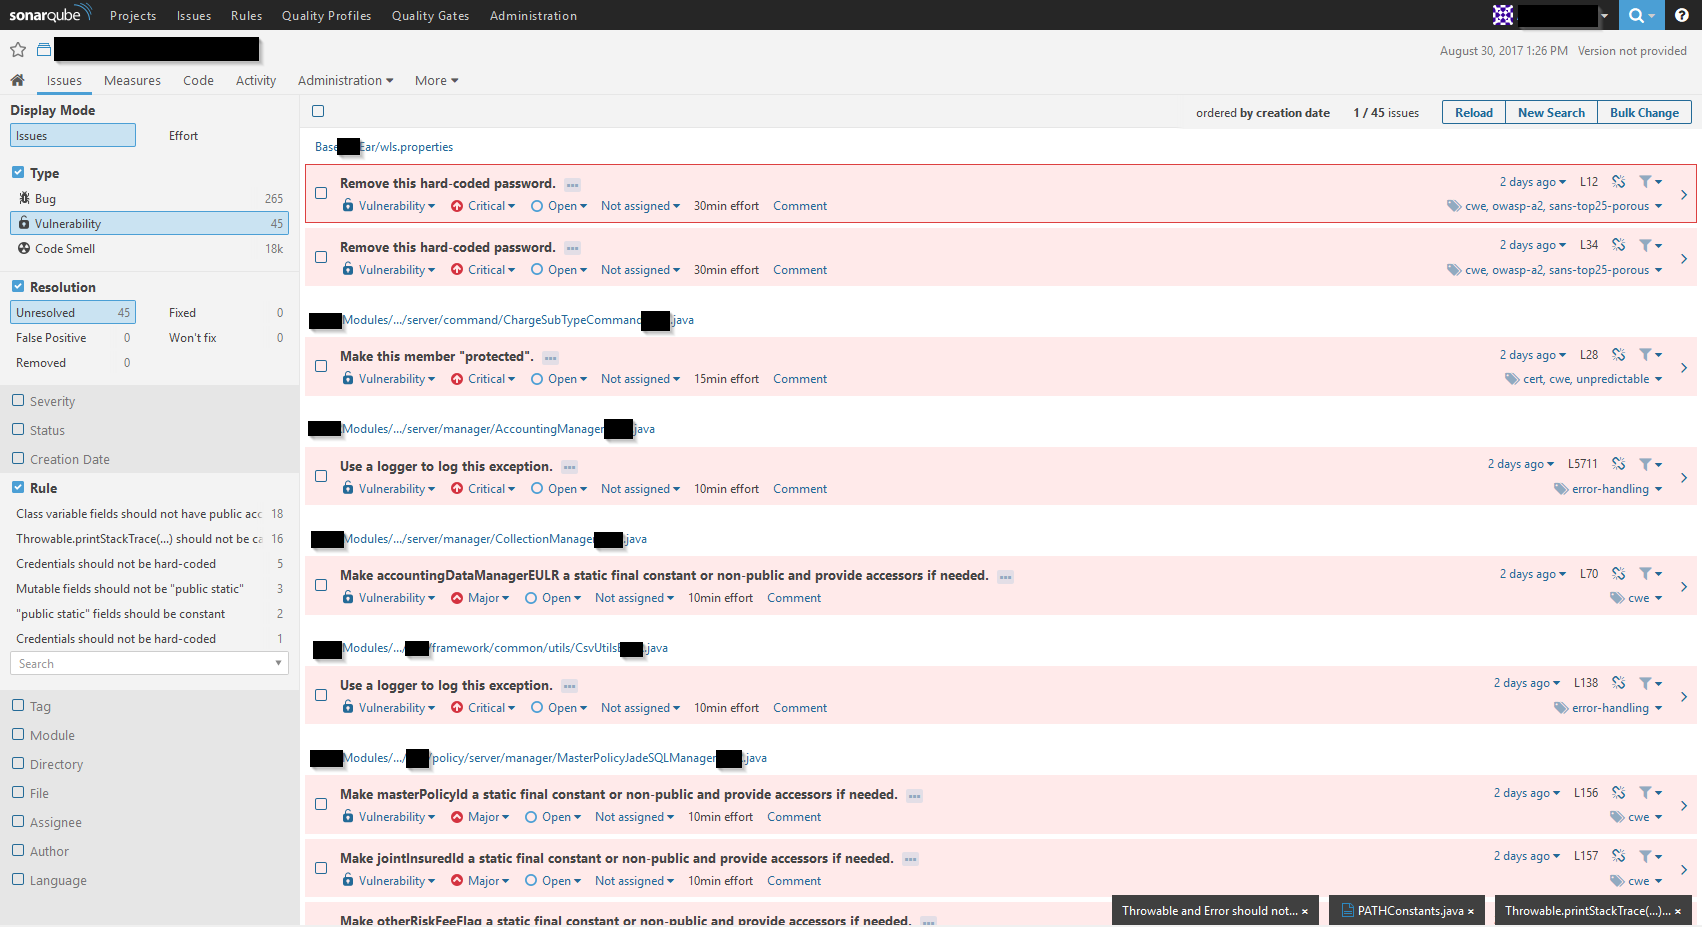
\includegraphics[width=\paperwidth]{images/sonar_sec_audit}}
	\caption{Extrait des résultats de sécurité du scanner Sonar}
	\label{fig:sonar_sec}
\end{figure}

C'est durant l'audit que j'ai majoritairement utilisé Sonar, mais les scripts de CI qui étaient en plus avant mon arrivée chez Alter Frame incorporaient déjà des analyses Sonar effectuées sur le code. C'est d'ailleurs de ce fait (mon tuteur ayant déjà de l'expérience avec ce logiciel) ainsi que du faible nombre de concurrents gratuits\cite{squale} que nous avons choisi d'utiliser Sonar dans ce cas de figure.

\subsubsection{JMeter \& SoapUI}
Ces deux outils, de même que ZAP, avaient déjà été utilisés lors des itérations précédentes de l'audit, et les conserver permettait de comparer facilement les résultats que nous obtiendrions avec les résultats antérieurs. Aussi, en l'absence de raison de ne \emph{pas} les conserver, nous les avons conservés.

SoapUI\cite{soapui} est un outil de test pour applications REST ou SOAP. L'application auditée utilisait le protocole SOAP, et SoapUI nous a servi à modifier et rejouer des requêtes isolées, sans tester les performances de l'application mais pour en saisir le fonctionnement et préparer le véritable test, en plus de vérifier que nous avions bien les droits pour réaliser toutes les opérations prévues.

JMeter est un outil de test de performances pour applications web en général. Le panel de fonctionnalités qu'il offre est extrêmement large (et en conséquence, sa prise en main est loin d'être triviale) et nous n'en avons utilisé qu'une partie : configurer JMeter comme proxy pour enregistrer un cas d'utilisation typique qui servira de scénario de test (on peut voir les différentes étapes d'un tel scénario dans l'interface de JMeter dans la figure~\ref{fig:jmeter}), puis rejouer celui-ci en boucle et plusieurs fois en parallèle pour tester les limites de l'application.
\begin{figure}
  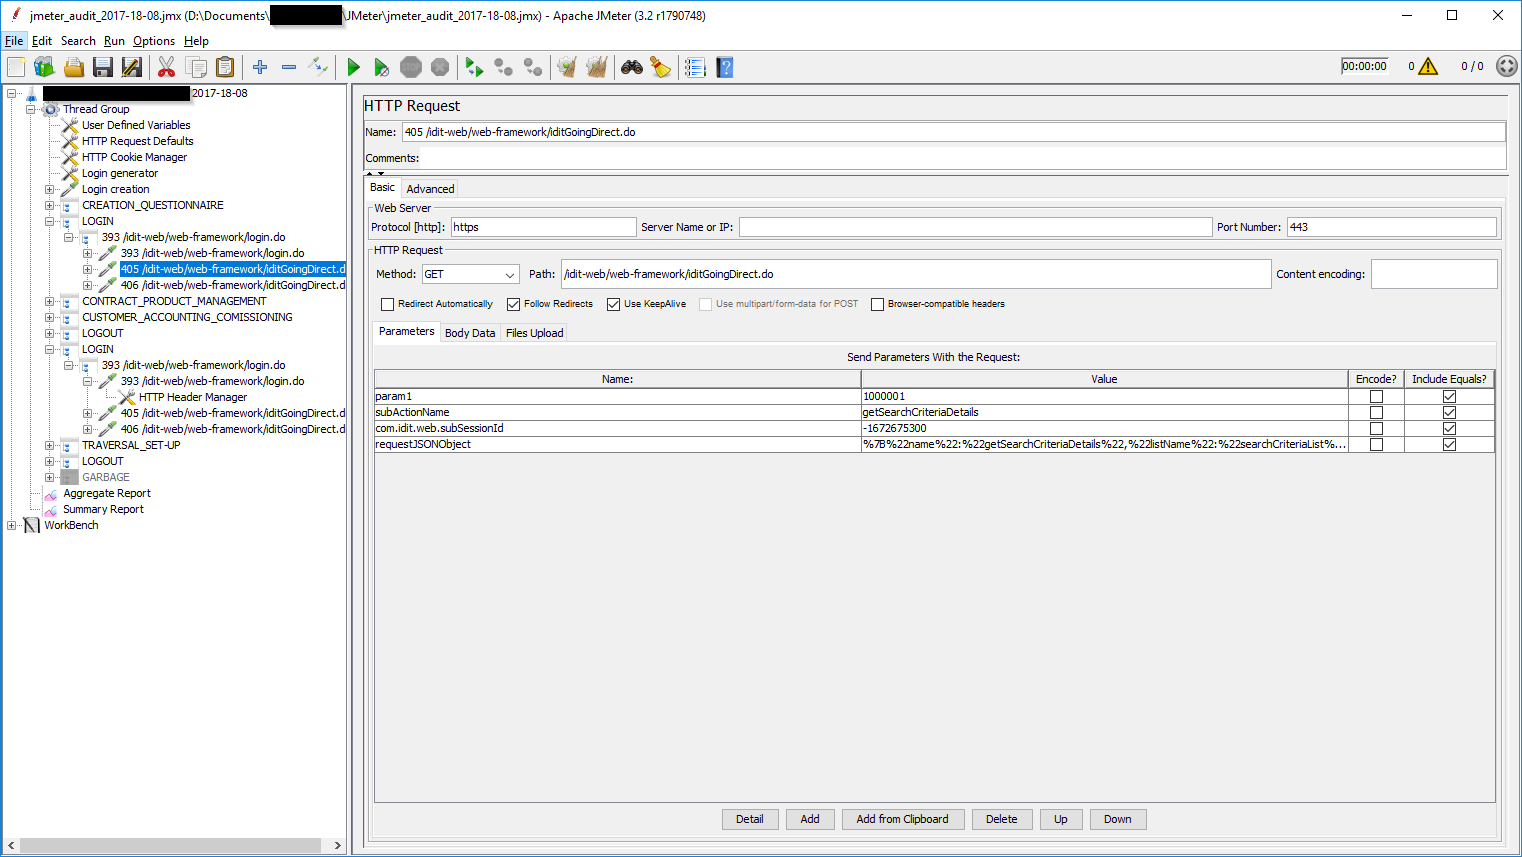
\includegraphics[width=\linewidth]{images/jmeter}
  \caption{JMeter, une fois configuré}
  \label{fig:jmeter}
\end{figure}

%TODO: ajouter un screen de JMeter
%%% Local Variables:
%%% mode: latex
%%% TeX-master: "../M2FSI-rapport-LEONARDI-alexandre"
%%% End:
